\chapter{Claude Shannon and data compression}
\label{chap-shannon}
\chapteroverview{How many bits are needed to store a message without losing information? Shannon's theory relates this question to the probabilities of the symbols in the message. Starting from a small grayscale image, we introduce binary codes, explain unambiguous decoding, and derive the role of entropy in compression.}

\section{Digital data and coding}
Text, sound, images and video are stored and transmitted as sequences of bits: binary digits $\RE{0}$ and $\RE{1}$. Before this binary representation is chosen, the data are described by \emph{symbols}: letters in a text, for instance, or pixel values in an image. A lossless compression method seeks a compact binary representation of a sequence of symbols from which the original sequence can be recovered exactly.

Shannon's work~\cite{Shannon1948,shannon1949} established fundamental limits for representing and communicating information. It is useful to distinguish the operations involved:
\begin{itemize}
\item \emph{Sampling} records a continuous signal at selected locations or times. \emph{Quantization} then replaces its values by elements of a finite set.
\item \emph{Source coding}, the subject of this chapter, seeks a compact representation of the resulting symbols.
\item \emph{Channel coding} adds redundancy to detect or correct transmission errors. Protection against malicious alteration is a separate security problem.
\end{itemize}
Sampling and quantization may discard information. The coding studied here is lossless relative to the symbols that have already been acquired. This distinction matters when discussing the compression of photographs or sound recordings.

\section{Encoding and decoding}
\subsection{A small grayscale image}
A grayscale image is an array of pixels. For simplicity, consider four possible values: $\BL{0}$ for black, $\BL{1}$ for dark gray, $\BL{2}$ for light gray and $\BL{3}$ for white. The same ideas apply to a larger alphabet, such as the 256 values of an eight-bit grayscale image, and to the channels of a color image.

Figure~\ref{fig-image-zoom} shows a flower and a magnified $5\times5$ patch. Reading its 25 values in the indicated order gives
\begin{equation}\label{eq-pixel-message}
 (\BL{0,1,3,2,0,3,2,2,1,2,2,1,1,2,2,2,1,1,2,2,2,1,1,2,1}).
\end{equation}
\myfig{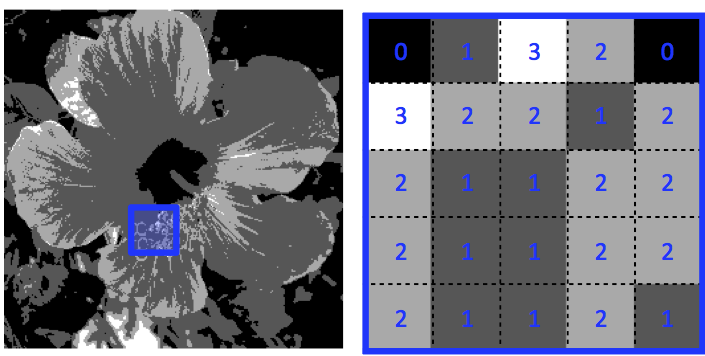
\includegraphics[width=.60\linewidth]{codage/codage-pxl}}
{fig-image-zoom}{A four-level grayscale image and a magnified $5\times5$ patch.}

\subsection{Fixed-length coding}
A \emph{codeword} is the bit string assigned to a symbol. We require nonempty codewords unless the message length is known in advance. One possible assignment is
\[
 \BL{0}\mapsto\RE{00},\qquad \BL{1}\mapsto\RE{01},\qquad
 \BL{2}\mapsto\RE{10},\qquad \BL{3}\mapsto\RE{11}.
\]
All four codewords have length two, so this is a \emph{fixed-length} code, also called a uniform code. Encoding a message means concatenating its codewords. For example,
\[
 (\BL{0,1,3})\longmapsto(\RE{00},\RE{01},\RE{11})\longmapsto\RE{000111}.
\]
The complete message~\eqref{eq-pixel-message} becomes
\[
 \RE{\mathtt{00011110001110100110100101101010010110101001011001}}.
\]
Its total length is $\overline{L}=25\times2=50$ bits. This count concerns the encoded pixel values; a file may also store dimensions, a coding table and other metadata.

For an alphabet of $N\ge2$ symbols, a fixed-length binary code of length $\ell$ exists precisely when $2^\ell\geq N$: there must be at least as many distinct bit strings as symbols. The smallest possible length is therefore
\[
 \ell=\lceil\log_2 N\rceil.
\]
When $N=2^\ell$, no bit strings are left unused. For $N=8$, for example, the codewords have length $\ell=3$ and are\[000,\ 001,\ 010,\ 011,\ 100,\ 101,\ 110,\ 111.\]

The base-two logarithm is defined for $x>0$ by $\log_2x=\ln x/\ln2$. It satisfies $\log_2(1/x)=-\log_2x$; in particular,
\[
 \log_2(1/4)=-\log_2 4=-2.
\]
The ceiling in the formula for $\ell$ is essential when $N$ is not a power of two.

\subsection{Variable-length coding}
A code can use fewer bits on average by assigning shorter words to frequent symbols. Consider
\begin{equation}\label{eq-prefix-example}
 \BL{0}\mapsto\RE{001},\qquad \BL{1}\mapsto\RE{01},\qquad
 \BL{2}\mapsto\RE{1},\qquad \BL{3}\mapsto\RE{000}.
\end{equation}
Now $(\BL{0,1,3})$ becomes $\RE{00101000}$. The complete message becomes
\[
 \RE{\mathtt{001010001001000110111010111101011110101101}},
\]
which has 42 bits. The \emph{average length per symbol} is
\[
 L=\frac{\overline{L}}{25}=\frac{42}{25}=1.68\ \text{bits}.
\]
This code improves on the fixed-length code for this particular message. It need not do so for every message: a sequence consisting mainly of symbols $\BL{0}$ and $\BL{3}$ would require nearly three bits per symbol.

\subsection{Prefix codes and unambiguous decoding}
A code is \emph{uniquely decodable} if two different finite symbol sequences never produce the same bit string. Fixed-length codes with distinct codewords have this property: split the message into blocks of $\ell$ bits, then read the coding table backwards.

Distinct codewords alone are not sufficient for a variable-length code. For example, the assignment
\[
 \BL{0}\mapsto\RE{0},\quad \BL{1}\mapsto\RE{10},\quad
 \BL{2}\mapsto\RE{110},\quad \BL{3}\mapsto\RE{101}
\]
is ambiguous because $\RE{1010}=\RE{10}\,\RE{10}=\RE{101}\,\RE{0}$ represents either $(\BL{1,1})$ or $(\BL{3,0})$.

A sufficient condition for unique decoding is that no codeword be a proper prefix of another. Such a code is called a \emph{prefix code}. The code~\eqref{eq-prefix-example} has this property. Its words can be recognized as soon as their last bit is read:
\[
 \underbrace{\RE{001}}_{\BL{0}}\;
 \underbrace{\RE{01}}_{\BL{1}}\;
 \underbrace{\RE{000}}_{\BL{3}}\;
 \underbrace{\RE{1}}_{\BL{2}}\;\cdots.
\]
The spaces shown here explain the decoding; they are not transmitted.

The prefix condition is sufficient, but not necessary. The code $A\mapsto0$, $B\mapsto01$ is uniquely decodable although $0$ prefixes $01$. Every $1$ must be paired with its preceding $0$, so the complete message has only one parsing. A decoder must nevertheless look ahead after reading a $0$ to decide whether it represents $A$ or begins $B$. More general non-prefix codes can require delayed decisions or backtracking; prefix codes avoid this difficulty.

\subsection{Codes as binary trees}\label{sec-arbres}
The empty word is the root of a binary tree. Appending a $0$ or a $1$ selects its left or right child. A word of length $\ell$ lies at depth $\ell$, so the complete tree of depth $\ell$ contains $2^\ell$ leaves and $\ell+1$ levels, including the root.

\myfig{\tabDeux{
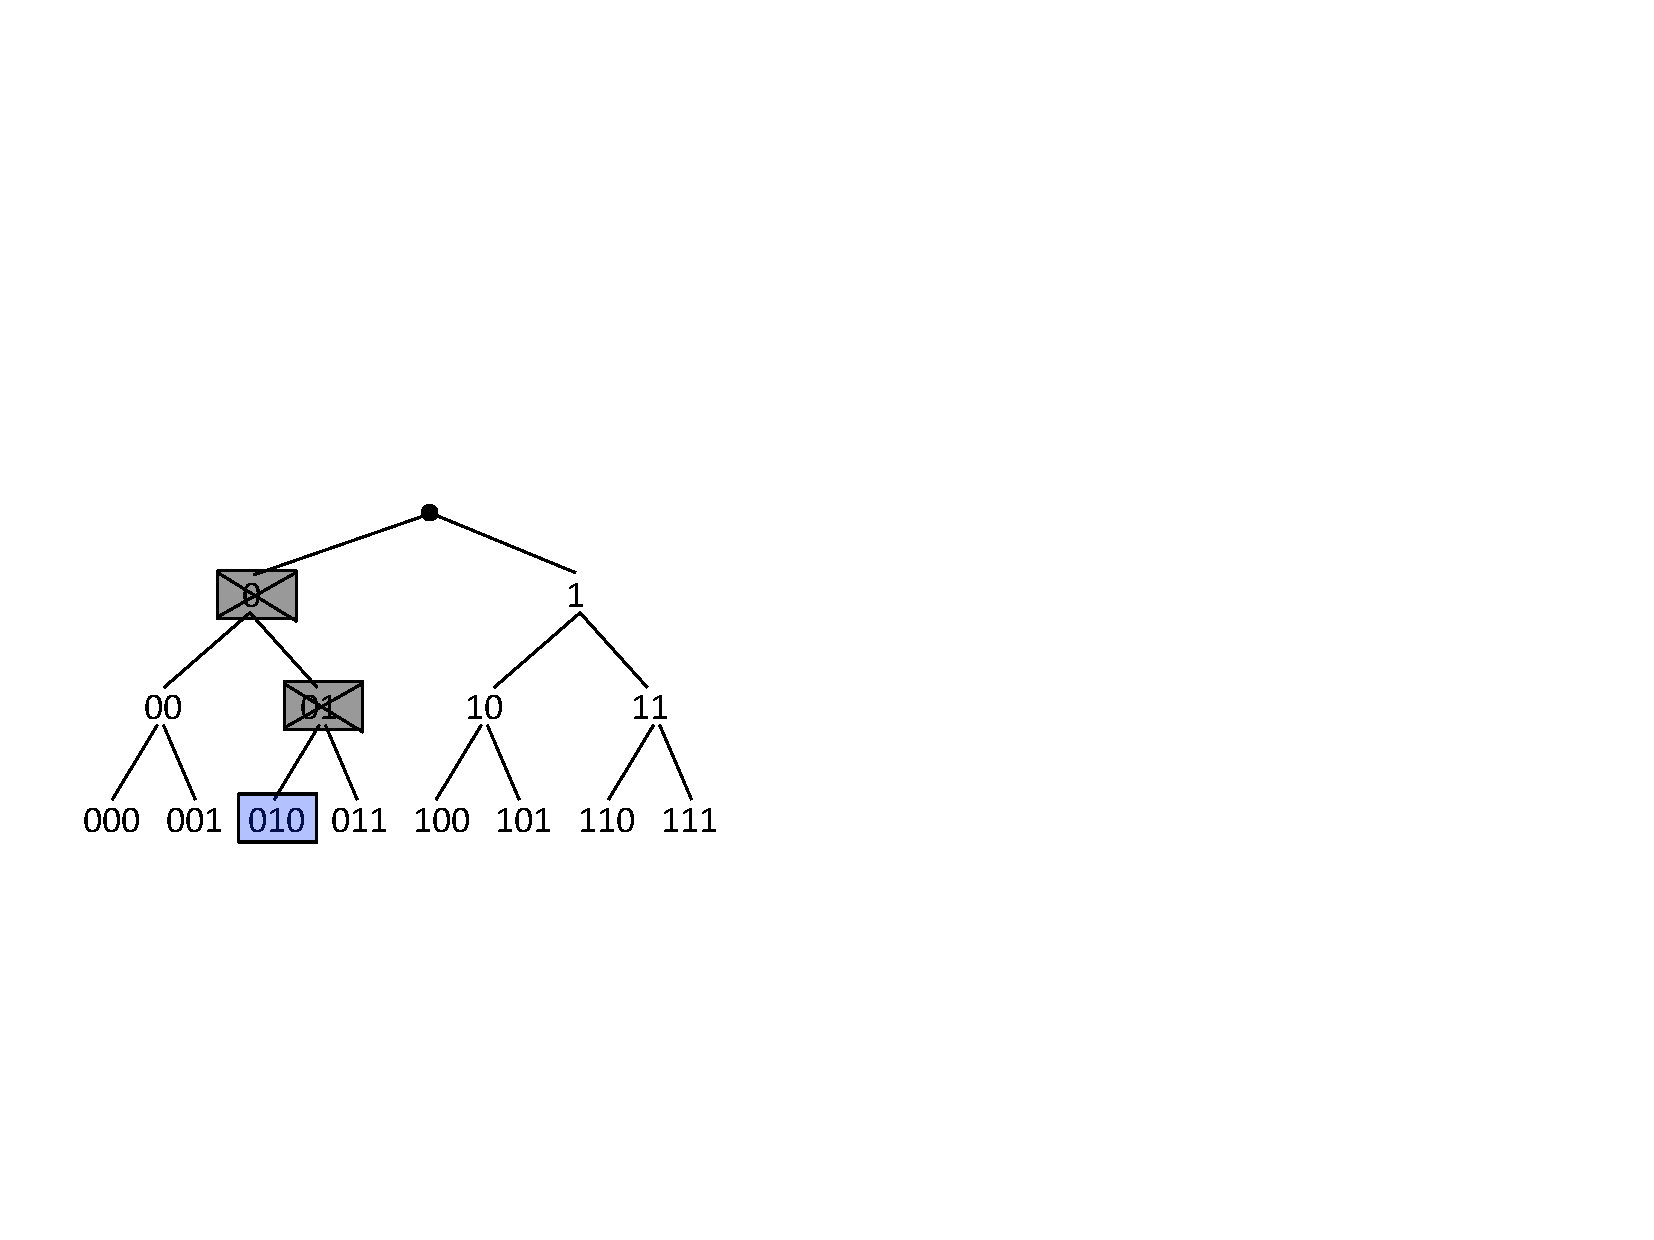
\includegraphics[width=.42\linewidth]{arbres/codage-prefixe}&
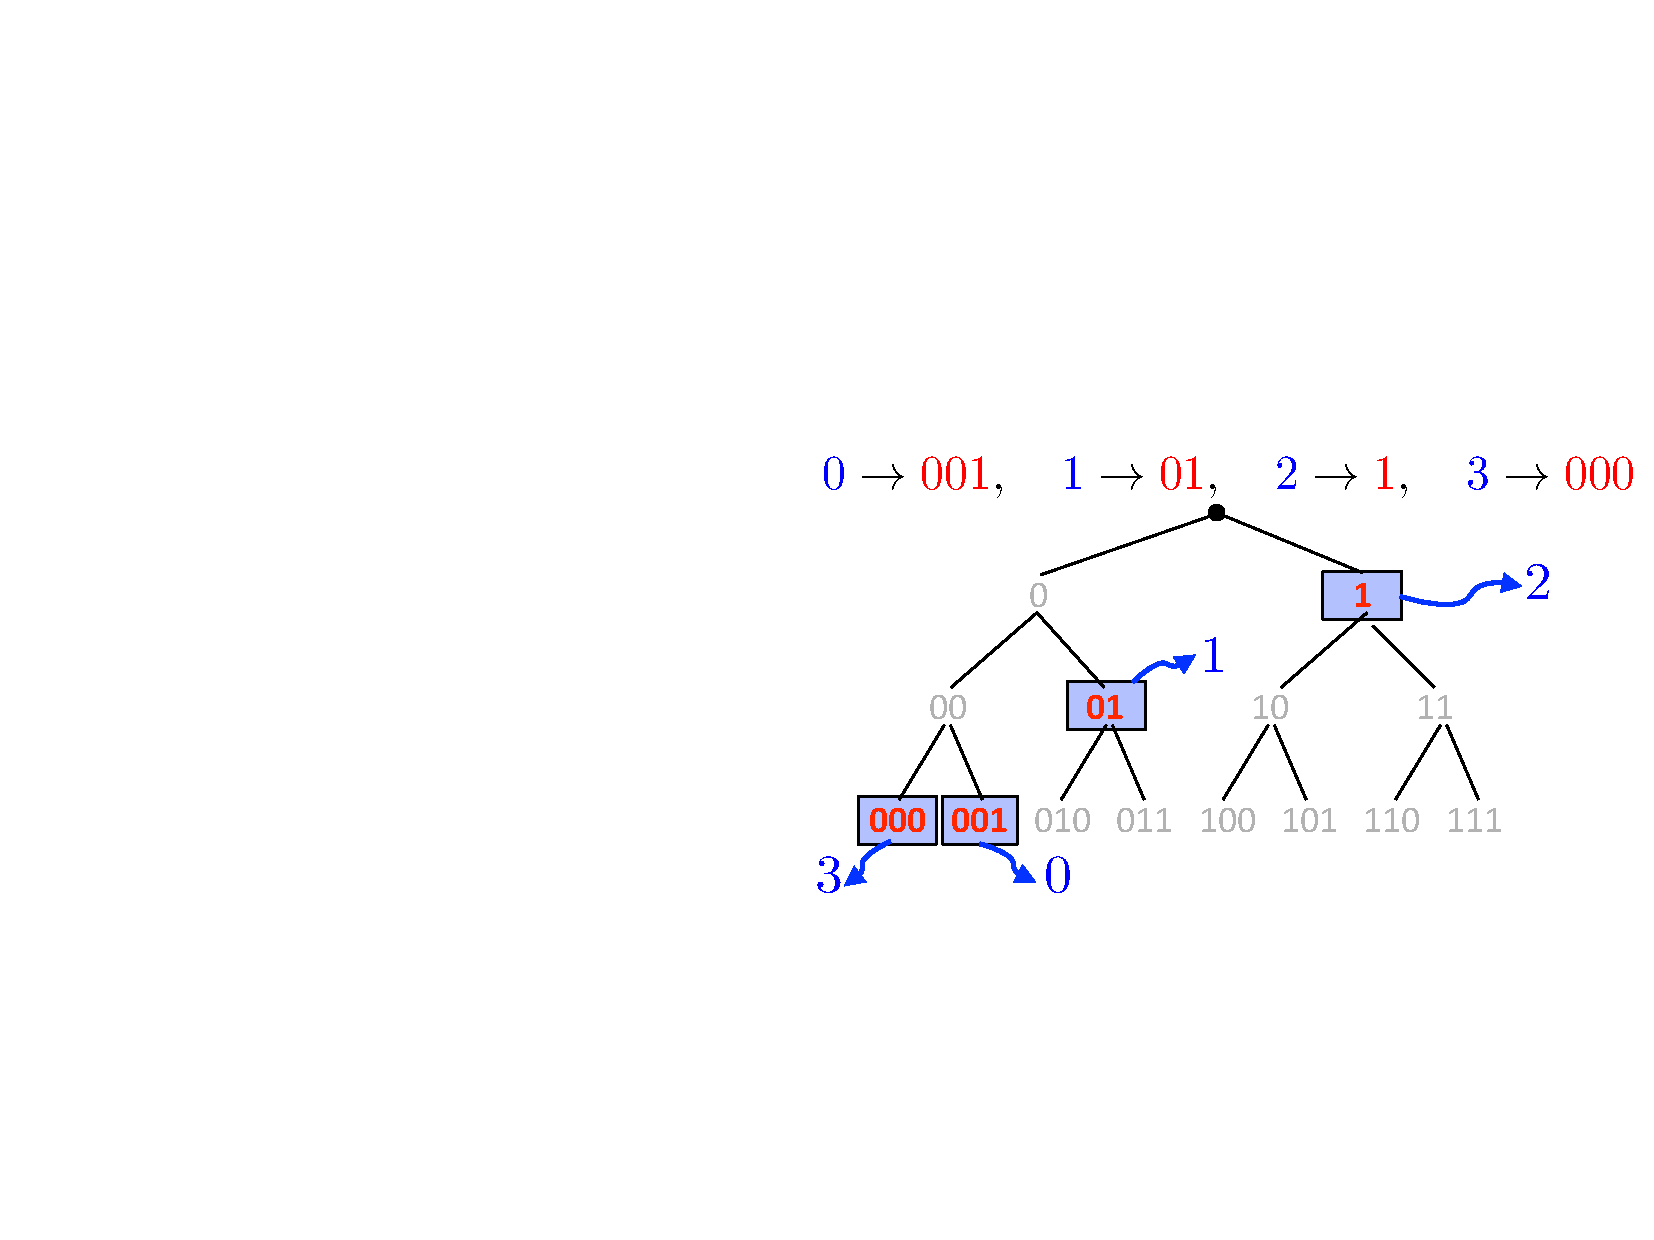
\includegraphics[width=.42\linewidth]{arbres/arbre-exemple}}}
{fig-trees}{The complete binary tree to depth three (left) and the subtree of a prefix code (right).}

For a prefix code, no selected codeword is an ancestor of another. The selected nodes are therefore leaves of the tree formed by their paths from the root. To decode, start at the root and follow one edge per bit. On reaching a codeword leaf, output its \emph{symbol} and return to the root. This procedure explains why prefix decoding is immediate and unambiguous.

\section{Entropy and the Shannon bound}
\subsection{A probabilistic model}
The quality of a code depends on the messages to which it is applied. A probabilistic model makes this dependence explicit. Let $V$ be a random symbol taking values in $\{0,\ldots,N-1\}$, with probabilities
\[
 p_v=\mathbb{P}(V=v),\qquad p_v\geq0,\qquad \sum_{v=0}^{N-1}p_v=1.
\]
The simplest model generates a sequence of independent symbols with this same distribution. Independence is an assumption about the source, not a property guaranteed by the coding algorithm.

For an observed message, probabilities can be estimated by \emph{empirical frequencies}. The message~\eqref{eq-pixel-message} contains 2 zeros, 9 ones, 12 twos and 2 threes. Its empirical distribution is
\[
 p=(2/25,\;9/25,\;12/25,\;2/25).
\]
Using these frequencies as probabilities is a modeling choice. If the decoder does not already know the chosen model or coding table, the information needed to describe it must also be transmitted.

\subsection{Entropy}
The \emph{entropy} of $V$, measured in bits, is
\begin{equation}\label{eq-entropy}
 H(V)=-\sum_{v=0}^{N-1}p_v\log_2p_v.
\end{equation}
A symbol with probability $p_v>0$ carries the information $-\log_2p_v$. Entropy is the average of this quantity. The convention $0\log_2 0=0$ means that impossible symbols contribute nothing; it agrees with $\lim_{x\downarrow0}x\log_2x=0$.

Since $-\log_2p_v\geq0$, entropy is nonnegative. More precisely,
\[
 0\leq H(V)\leq\log_2N.
\]
The endpoints describe two useful models:
\begin{itemize}
\item \textbf{No uncertainty.} If $p_1=1$, every symbol equals $1$ and $H(V)=0$. The message is a sequence of ones.
\item \textbf{Maximum uncertainty.} If $p_v=1/N$ for all $v$, then $H(V)=\log_2N$. With four equally likely symbols, this is two bits. A random message from this model need not contain exactly the same number of each symbol.
\item \textbf{An intermediate case.} For the empirical distribution above,
\[
 H(V)=-2\frac{2}{25}\log_2\frac{2}{25}
       -\frac{9}{25}\log_2\frac{9}{25}
       -\frac{12}{25}\log_2\frac{12}{25}
       \simeq1.6219\ \text{bits}.
\]
\end{itemize}
\myfig{\tabTrois{
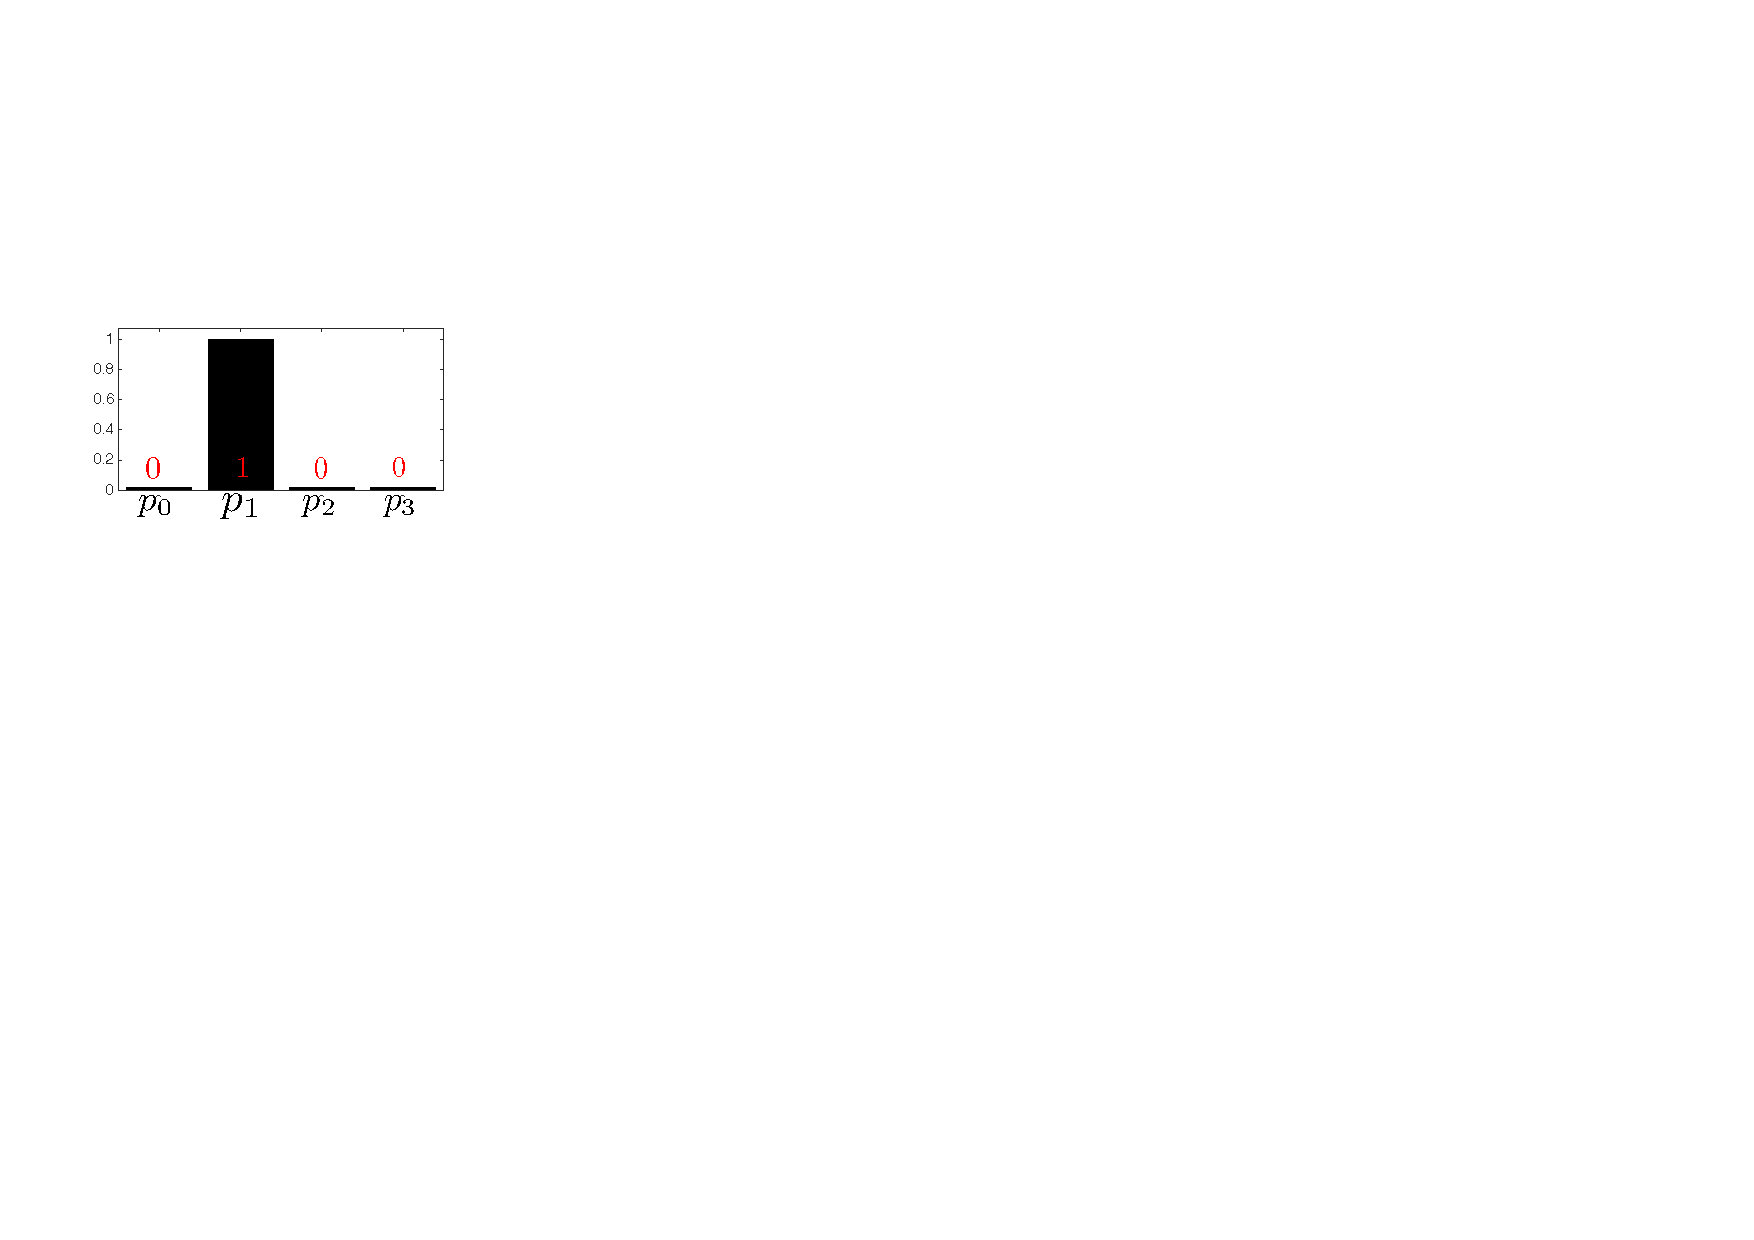
\includegraphics[width=.30\linewidth]{entropie/histo-1}&
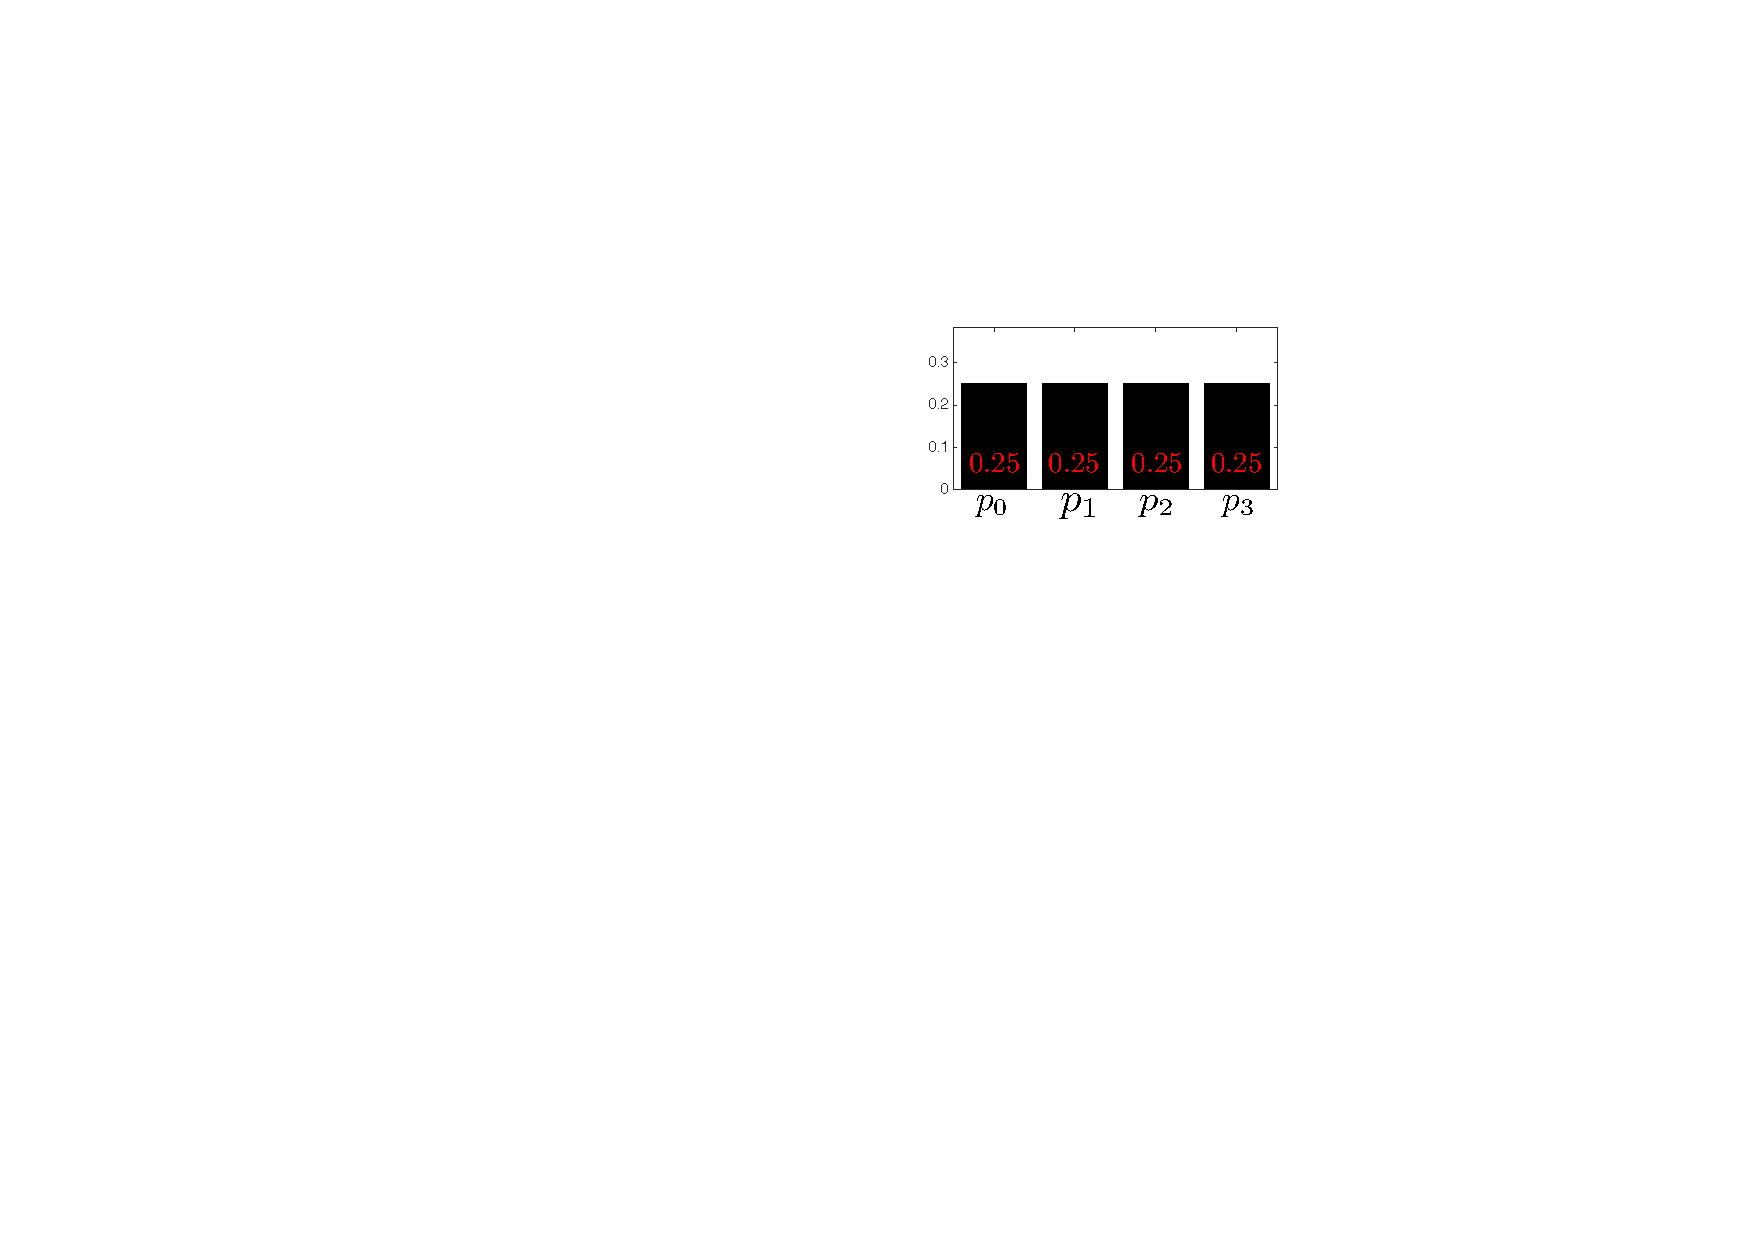
\includegraphics[width=.30\linewidth]{entropie/histo-3}&
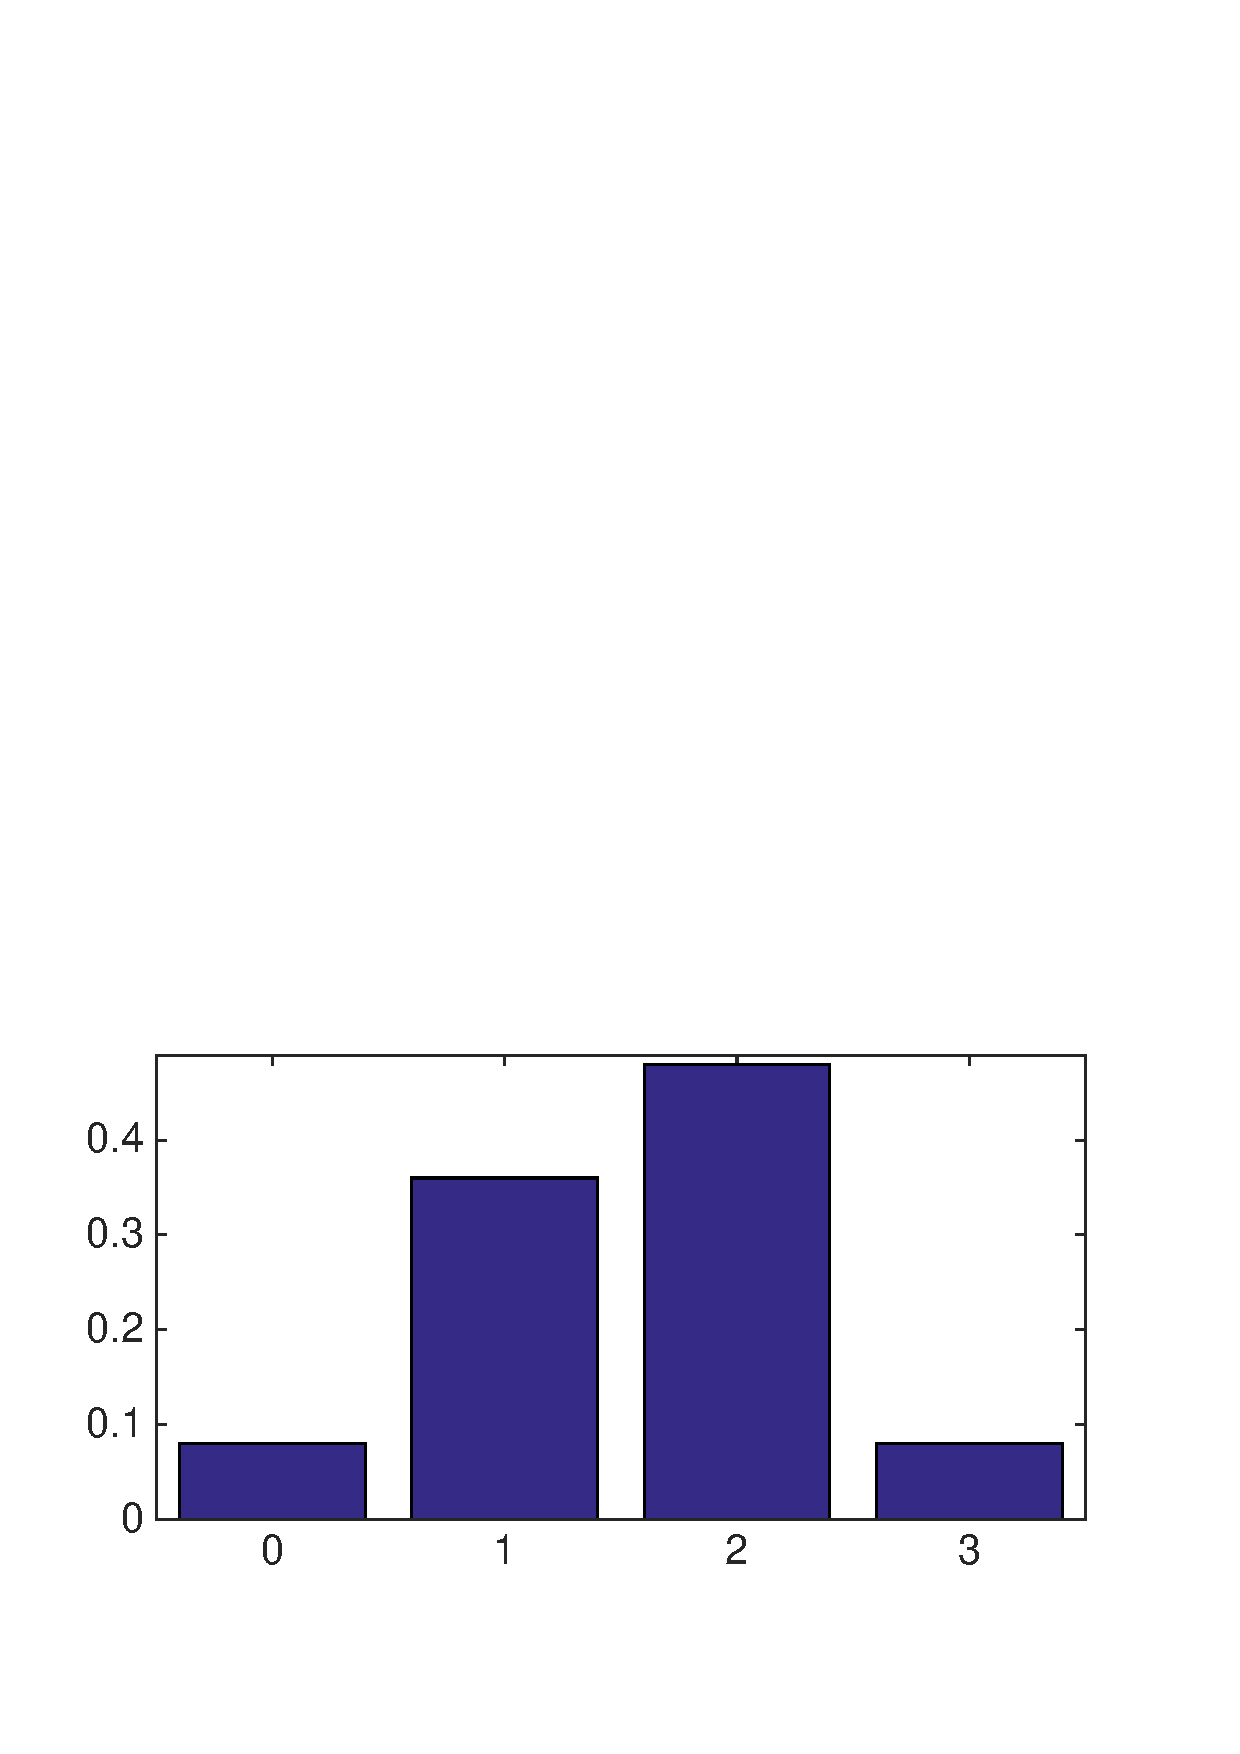
\includegraphics[width=.30\linewidth]{entropie/histo-sub}\\
$H(V)=0$&$H(V)=2$&$H(V)\simeq1.62$}}
{fig-histo-entropy}{A deterministic distribution, the uniform distribution on four symbols, and the empirical distribution of the 25-pixel message.}

\subsection{Expected code length}
Let $c_v$ be the codeword for $v$ and $\ell_v$ its length. The expected number of bits per symbol is
\[
 L(c)=\mathbb{E}[\ell_V]=\sum_v p_v\ell_v.
\]
For the code~\eqref{eq-prefix-example}, the lengths are $(3,2,1,3)$, hence
\[
 L(c)=\frac{2\times3+9\times2+12\times1+2\times3}{25}
     =\frac{42}{25}=1.68.
\]
If $p$ is the empirical distribution of a finite message, this formula is also its exact average code length. If $p$ is a source model, it is an expectation.

\subsection{The entropy lower bound}
Every binary prefix code satisfies the Shannon bound~\cite{Shannon1948}
\begin{equation}\label{eq-shannon-bound}
 H(V)\leq L(c).
\end{equation}
Here is a short proof. Let $m$ be the greatest codeword length. A word of length $\ell_v$ has $2^{m-\ell_v}$ descendants at depth $m$. Prefix-free words have disjoint sets of descendants, so
\[
 \sum_v2^{m-\ell_v}\leq2^m,
 \qquad Z\eqdef\sum_v2^{-\ell_v}\leq1.
\]
This is Kraft's inequality. Define $q_v=2^{-\ell_v}/Z$. Then $\sum_vq_v=1$ and $\ell_v=-\log_2q_v-\log_2Z$, which gives
\[
 \begin{aligned}
 L(c)-H(V)
 &=\sum_{v:p_v>0}p_v\log_2\frac{p_v}{q_v}-\log_2Z\\
 &\geq\sum_{v:p_v>0}p_v\log_2\frac{p_v}{q_v}\geq0.
 \end{aligned}
\]
The last sum is the Kullback--Leibler divergence. Its nonnegativity follows from $\ln t\leq t-1$: applying this to $t=q_v/p_v$ and summing yields $\sum p_v\ln(q_v/p_v)\leq\sum_{p_v>0}q_v-1\leq0$.

The bound concerns an \emph{average}; it does not impose $\ell_v\geq-\log_2p_v$ separately for each symbol. The real numbers $-\log_2p_v$ nevertheless suggest useful target lengths: a \emph{larger} probability gives a smaller target length. For a uniform distribution on $2^\ell$ symbols, the fixed-length code attains the bound exactly. For other alphabet sizes, integer codeword lengths can prevent equality.

\subsection{Huffman coding and blocks}
Huffman's algorithm~\cite{Huffman52} constructs a prefix code with minimum expected length for a given finite distribution. Symbols of probability zero are omitted from the effective alphabet. For a source with at least two positive-probability symbols, its length satisfies the strict upper bound
\[
 H(V)\leq L(c)<H(V)+1.
\]
One way to understand the upper bound is to round each target length up: $\ell_v=\lceil-\log_2p_v\rceil$. These lengths satisfy Kraft's inequality and can be realized by a prefix code. Their average is less than $H(V)+1$, and a Huffman code does at least as well.

To reduce the overhead per symbol, encode blocks of $n$ independent symbols. Their entropy is $H(V_1,\ldots,V_n)=nH(V)$, so a suitable block code has expected length $L_n$ satisfying
\[
 H(V)\leq\frac{L_n}{n}<H(V)+\frac1n.
\]
Thus the rate approaches entropy as the block length grows. Arithmetic coding~\cite{RissanenLangdon79} implements related ideas without storing an exponentially large table of block codewords. Finite messages still incur model, termination and numerical-precision overheads.

If a source has only one possible symbol, its entropy is zero. When this symbol and the message length are already known, no payload bits are needed. Requiring a nonempty codeword would instead spend at least one bit per symbol. The convention about framing and the effective alphabet must therefore be stated.

\subsection{Exploiting dependence between pixels}\label{sec-information-transform}
Neighboring pixels in an image are usually dependent. A symbol-by-symbol model ignores this structure. A useful remedy is to transform the data before coding them.

Index the $P$ pixels by $v_0,\ldots,v_{P-1}$ and define
\[
 d_i=v_i-v_{i-1},\qquad 1\leq i\leq P-1.
\]
Keep $v_0$ as well as the differences. The transformation
\[
 (v_0,\ldots,v_{P-1})\longmapsto(v_0,d_1,\ldots,d_{P-1})
\]
is bijective, since $v_i=v_0+\sum_{j=1}^i d_j$. In a nearly constant region, most differences are zero or small. For four-level pixels, they lie in $\{-3,-2,-1,0,1,2,3\}$.
\myfig{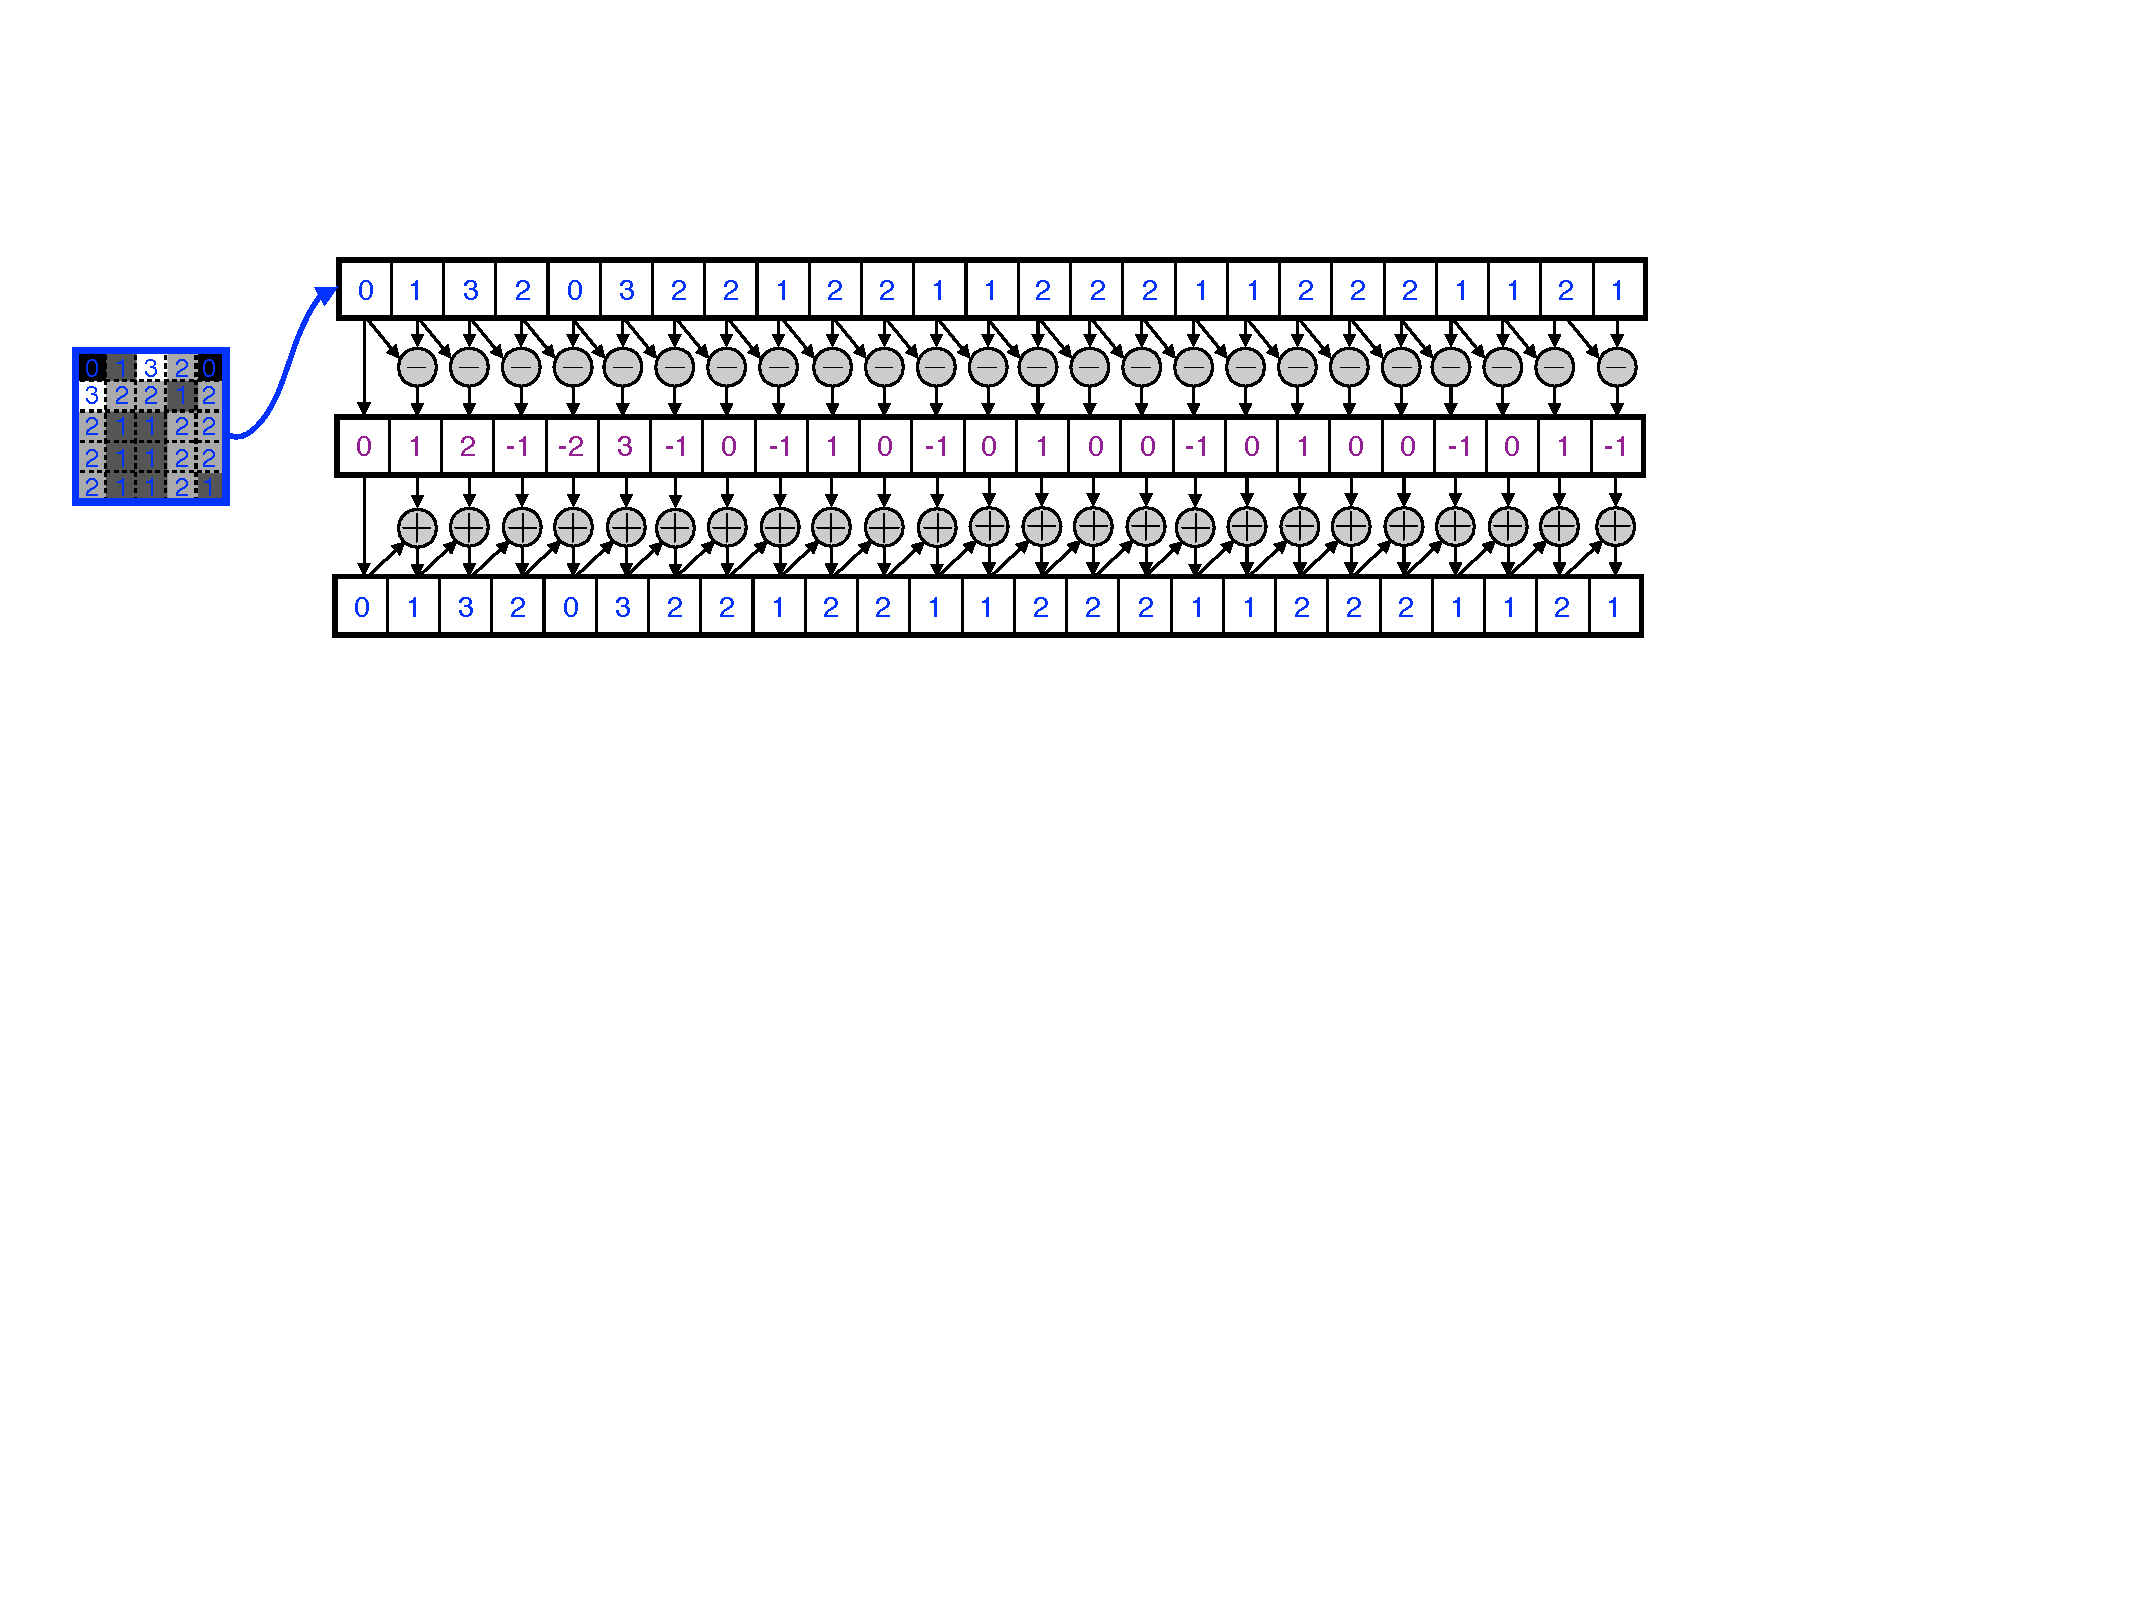
\includegraphics[width=\linewidth]{differences/differences}}
{fig-codage-differences}{Successive differences and reconstruction by cumulative summation, retaining the first pixel.}

For the flower example, the difference histogram is more concentrated than the pixel histogram. The empirical entropies and Huffman lengths shown in Figure~\ref{fig-entropy-differences} illustrate the resulting gain when values are coded separately. This gain is not guaranteed for every image.
\myfig{\tabTrois{
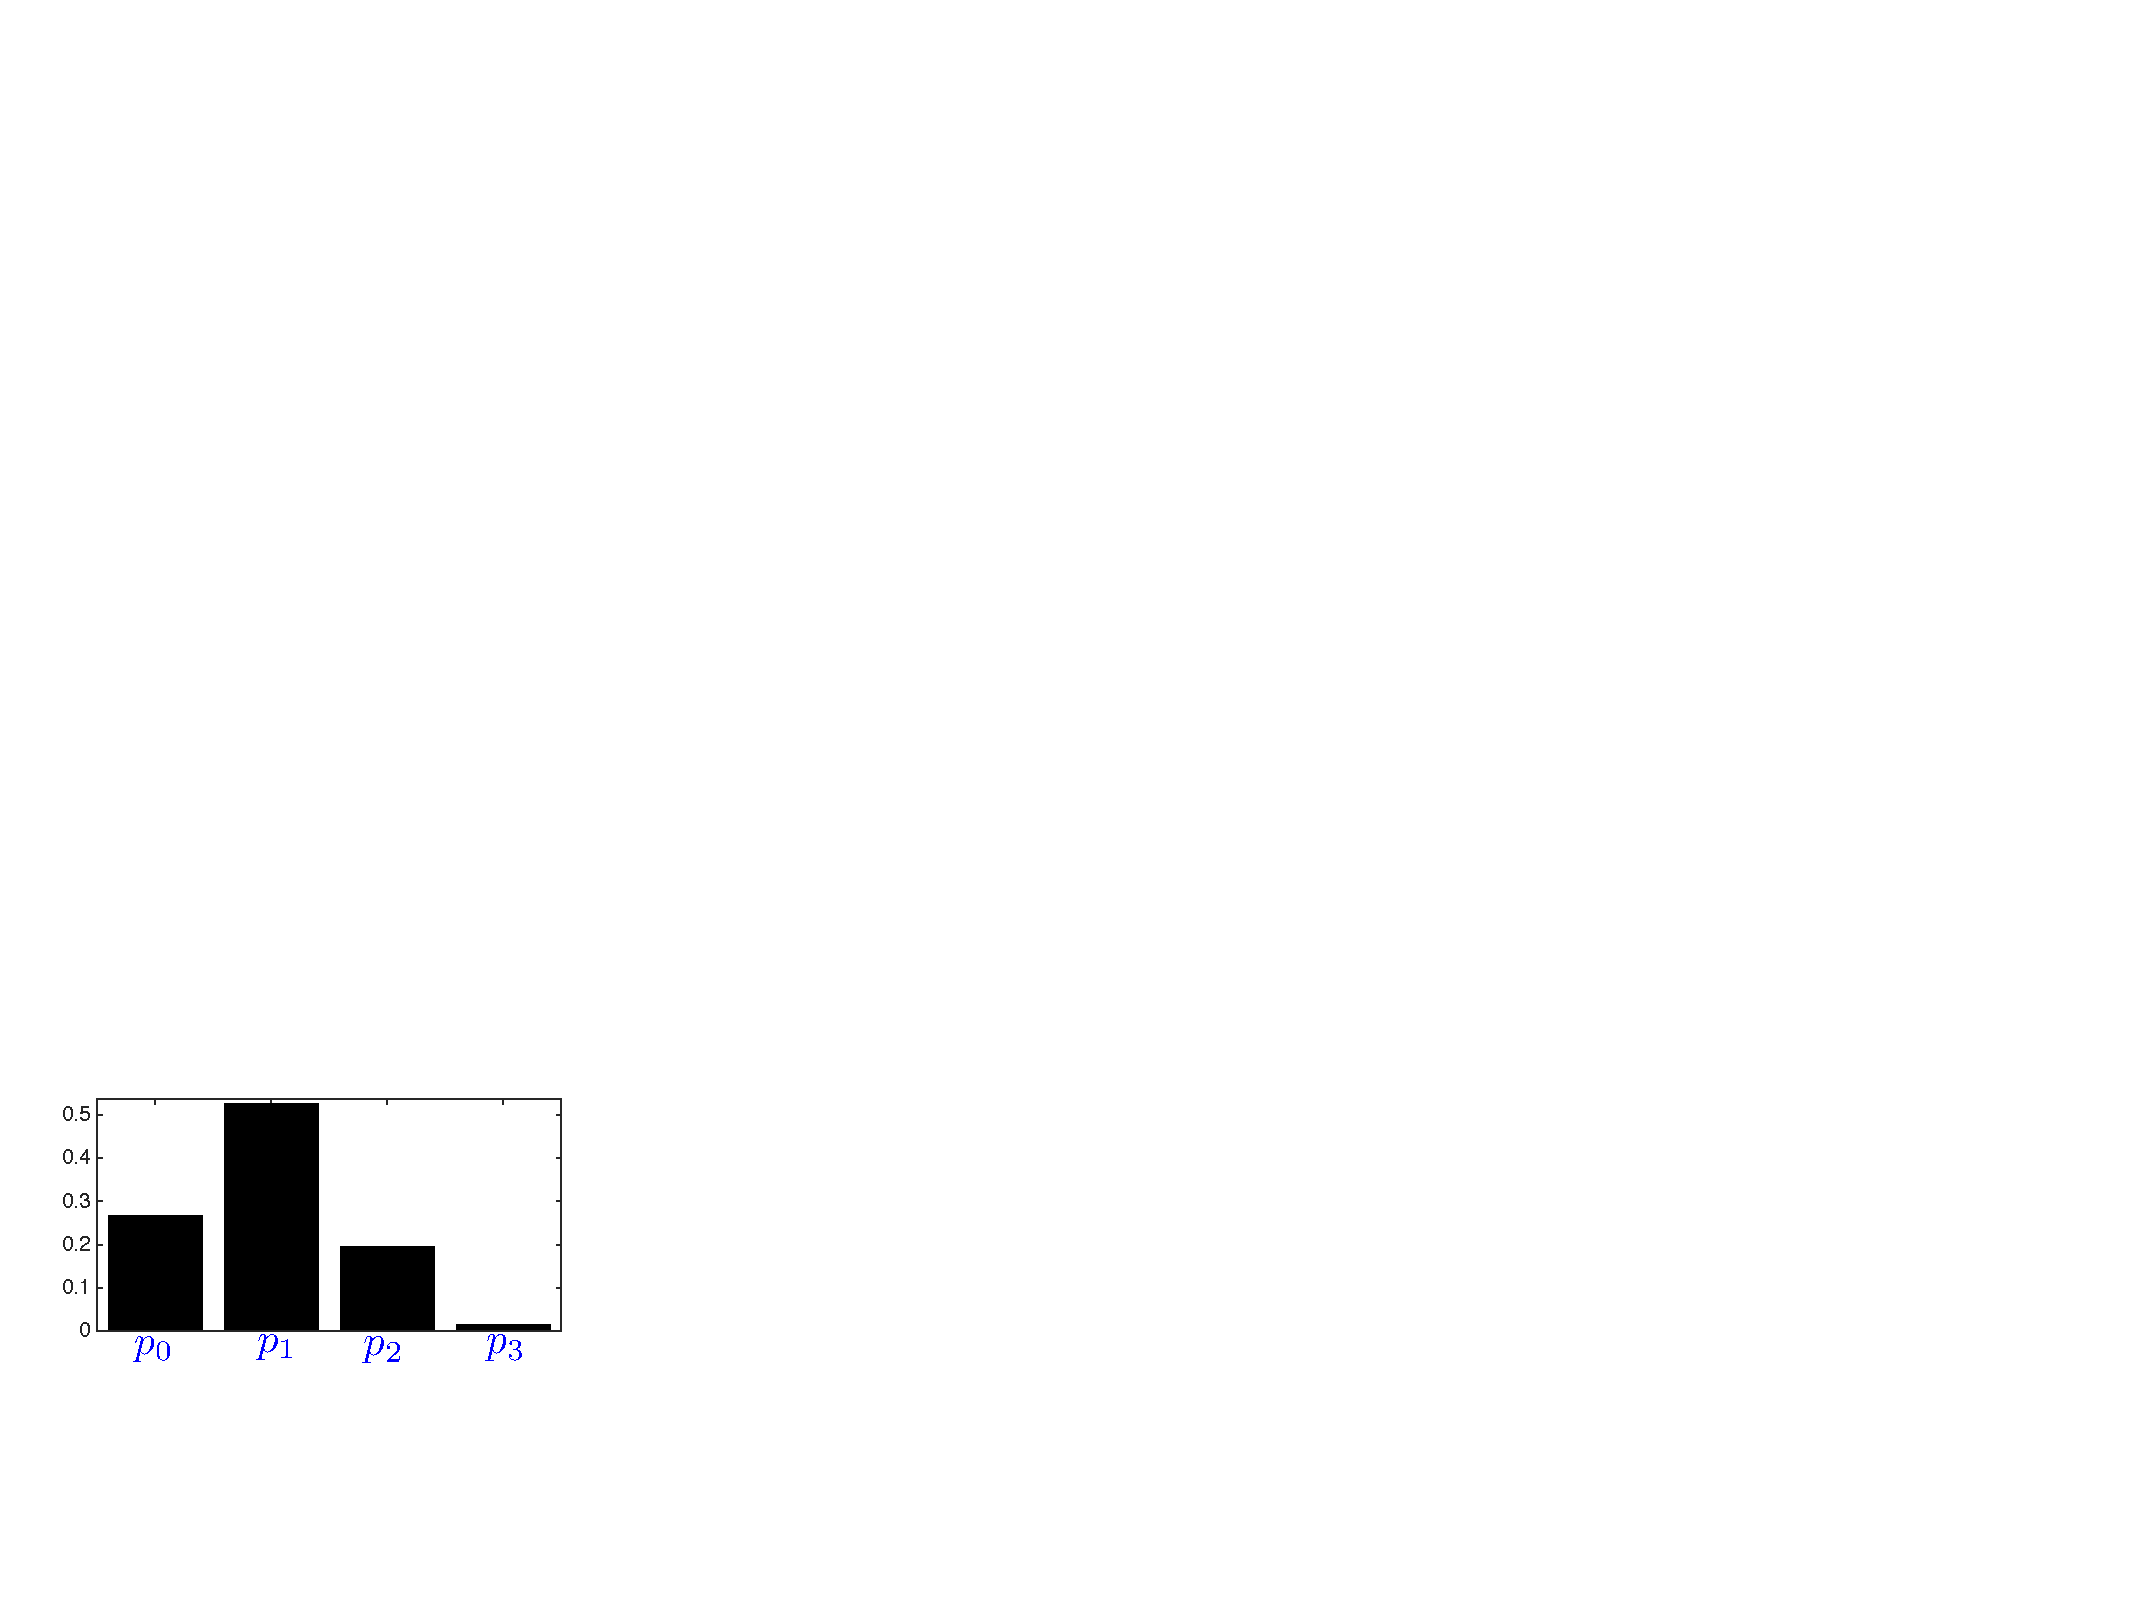
\includegraphics[width=.29\linewidth]{differences/histo-pix}&
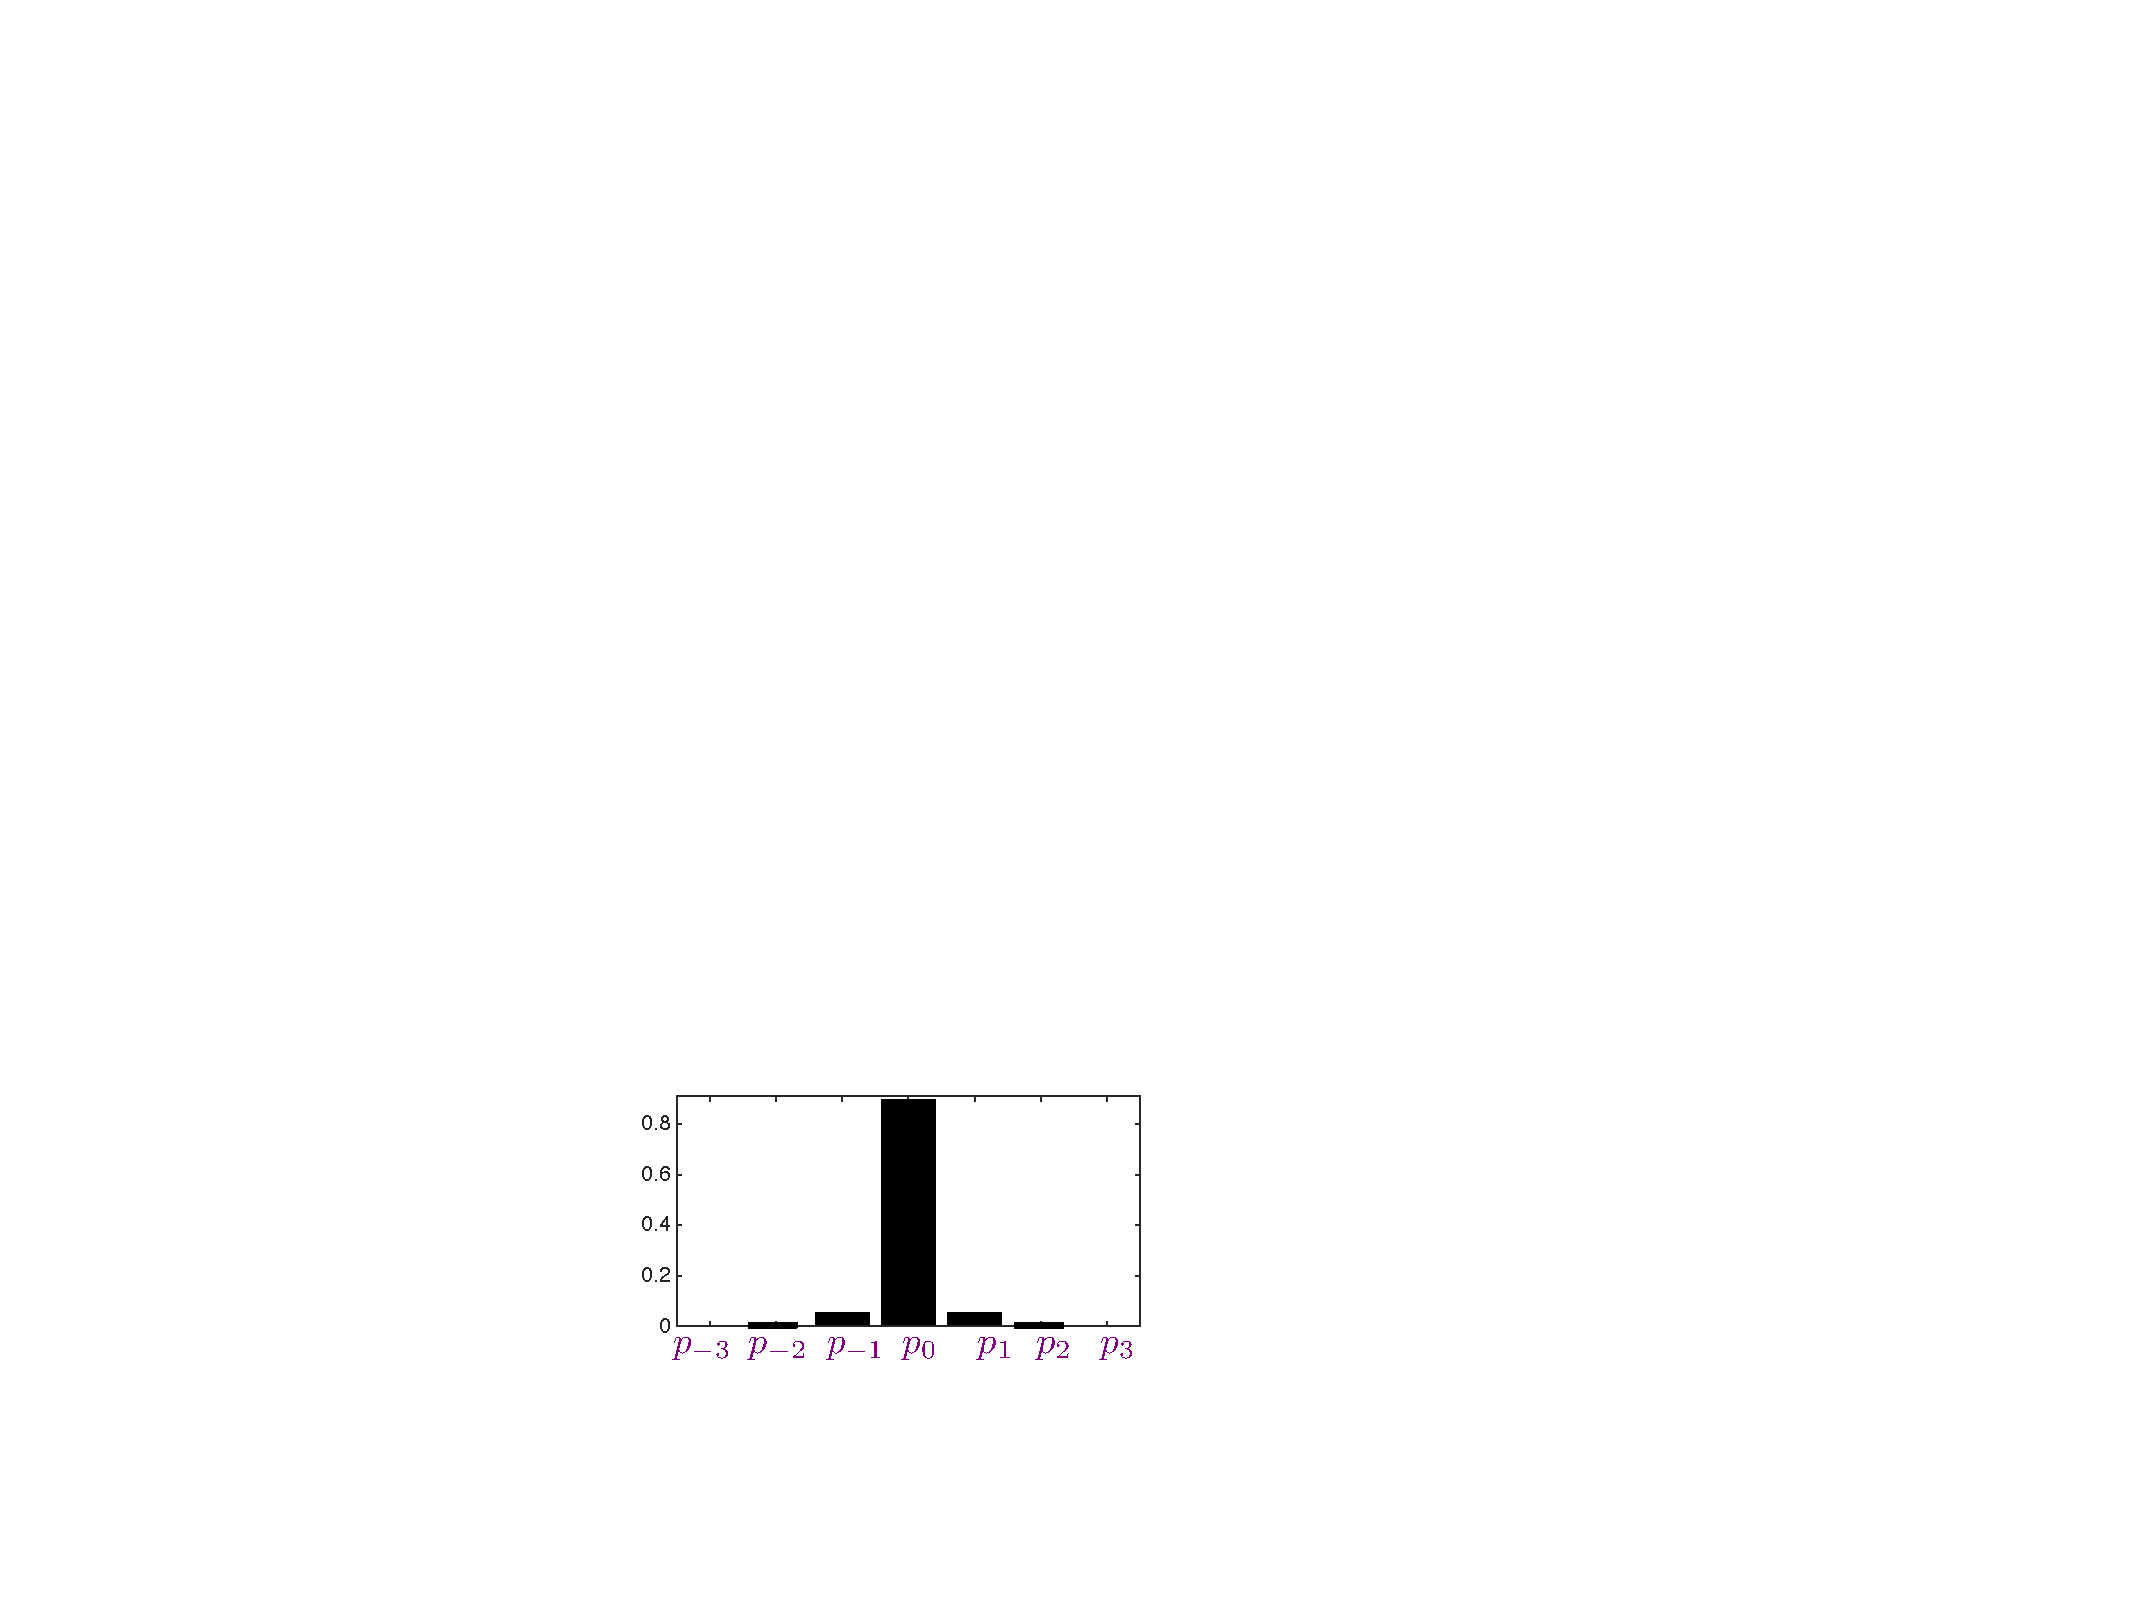
\includegraphics[width=.29\linewidth]{differences/histo-diff}&
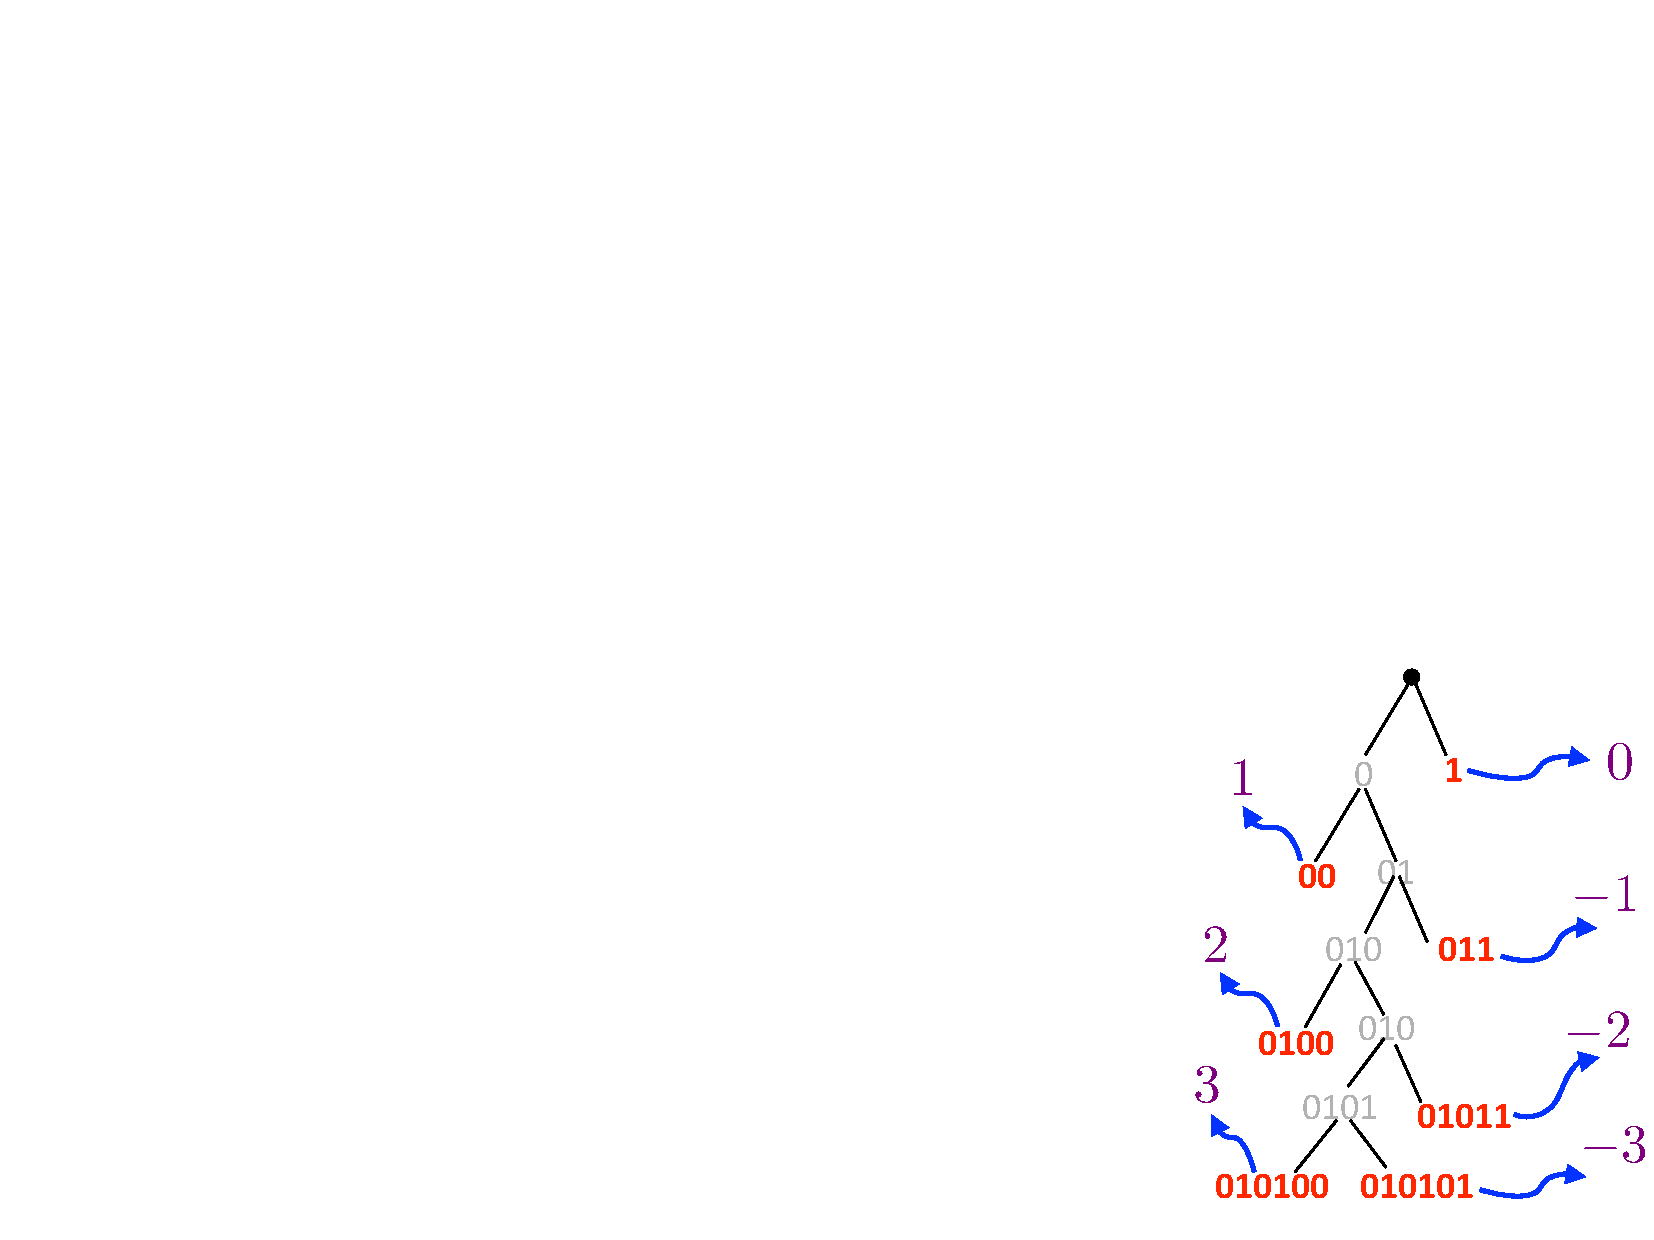
\includegraphics[width=.21\linewidth]{differences/arbre-difference}\\
$H\simeq1.54,\ L\simeq1.67$&$H\simeq0.61,\ L\simeq1.16$&\text{Prefix tree}}}
{fig-entropy-differences}{Pixel and difference histograms over the entire image, with a prefix-code tree for the differences.}

The displayed difference code is
\[
\begin{array}{c|rrrrrrr}
 d&-3&-2&-1&0&1&2&3\\\hline
 c_d&010101&01011&011&1&00&0100&010100
\end{array}
\]
and has an average length of approximately 1.16 bits per difference. Using the displayed rounded rates for a $256\times256$ image gives payload estimates of $16$ KiB for the two-bit fixed-length code, $13.36$ KiB for direct pixel coding, and $9.28$ KiB for difference coding. Here $1$ KiB is $1024$ bytes, or $8192$ bits. The initial pixel and coding-table overhead must be added to the last estimate.

A bijective transformation does \emph{not} reduce the joint entropy of the whole message. It can make separate-symbol models more effective by changing the marginal distributions and the dependence structure. The bound~\eqref{eq-shannon-bound} itself needs no independence assumption for a single random symbol; independence was used above to obtain the block identity $H(V_1,\ldots,V_n)=nH(V)$. For a dependent source, the joint entropy of the block is the relevant lower bound.

More advanced image codecs combine prediction or transforms with quantization and entropy coding. JPEG 2000, for example, uses wavelets and supports both lossless and lossy modes~\cite{mallat2009a-wav}. The same principle of exploiting dependence also applies to the letters of a text.

\paragraph*{Further reading.}
For further details on source coding, see~\cite{CoverThomas}, and~\cite{mallat2009a-wav} for signal and image processing. The original figure programs are available at \url{https://github.com/gpeyre/2016-shannon-theory}; related experiments appear in the Numerical Tours~\cite{2011-peyre-cise}.

\ifdefined\StandaloneChapter
\par\noindent\begin{minipage}{\linewidth}
\section*{Glossary}
\begin{multicols}{2}\small\raggedright
\begin{rs}
\gloss{Pixel}: a location in an image grid, or its stored value.
\gloss{Symbol}: an element of the finite alphabet to be encoded.
\gloss{Codeword}: the bit string assigned to one symbol.
\gloss{Code}: the assignment of codewords to symbols.
\gloss{Empirical distribution}: the observed relative frequencies of symbols.
\gloss{Histogram}: a graphical representation of these frequencies.
\gloss{Source model}: a probability law for the symbols or their sequences.
\gloss{Entropy}: the nonnegative average information $H(V)$, in bits.
\gloss{Average code length}: $L(c)=\sum_vp_v\ell_v$, in bits per symbol.
\end{rs}
\end{multicols}
\end{minipage}\par
\fi

\ifdefined\StandaloneChapter
\paragraph*{Acknowledgements.}
I thank Marie-Noëlle Peyré, Gwenn Guichaoua, François Béguin, Gérard Grancher, Aurélien Djament and François Sauvageot for their careful reading of the French text. The flower photograph is by Maïtine Bergounioux.
\fi
